
\lecture{Probability Rules}{probability-rules}
\section{Probability Rules}

\title{Probability Rules}
\subtitle{Calculating Probabilities}

%\author{Kelly Black}
%\institute{Clarkson University}
\date{15 January 2014}

\begin{frame}
  \titlepage
\end{frame}

\begin{frame}
  \frametitle{Outline}
  \tableofcontents[hideothersubsections,sectionstyle=show/hide]
\end{frame}



\iftoggle{clicker}{%
  \subsection{Clicker Quiz}


  \begin{frame}
    \frametitle{Clicker Quiz}

    I have a bag with eight marbles. Five marbles are red and three are
    blue. I pull one marble out at random. What is the probability that
    it is red?

    \begin{tabular}{l@{\hspace{3em}}l@{\hspace{3em}}l@{\hspace{3em}}l}
      A: 3/8 & B: 5/8 & C: 1
    \end{tabular}


  \end{frame}
}


\subsection{Examples}

\begin{frame}{Example}

  I roll a six-sided die. What is the probability that I roll a one?

  \only<2>%
  {
    \begin{eqnarray*}
      p(\underbrace{\mathrm{\color{red}{roll~a~one}}}_{\mathrm{an~\textbf{event}!}}) 
    \end{eqnarray*}
  }

  \only<3->%
  {
    I roll a six-sided die. What is the probability that I roll a one
    \textbf{or} a two?
  }

  \only<4->%
  {
    I roll a six-sided die. What is the probability that I roll an odd
    number?
  }

  \only<5->%
  {
    I roll a six-sided die. What is the probability that I roll an odd
    number \textbf{or} a number less than 3?
  }

  
\end{frame}


\begin{frame}{Something does not add up}

  \begin{eqnarray*}
    p(\mathrm{odd}) & = & \frac{3}{6}, \\
    p(\mathrm{number}<3) & = & \frac{2}{6}, \\
  \end{eqnarray*}

  \only<2->%
  {

    \begin{eqnarray*}
      p(\mathrm{odd}) + p(\mathrm{number}<3) & = & \frac{5}{6}, \\
      p(\mathrm{odd~or~\mathrm{number}<3}) & = & \frac{4}{6}.
    \end{eqnarray*}
    they are not the same!

  }

  
\end{frame}


\begin{frame}{Example}

  I roll a six-sided die. What is the probability that I roll an odd
  \textbf{and} a number less than 3?
  
\end{frame}

\begin{frame}{In General}

  What is $p(A~or~B)$?

  \only<1>{\includegraphics[width=5cm]{img/vennDiagram}}
  \only<2->{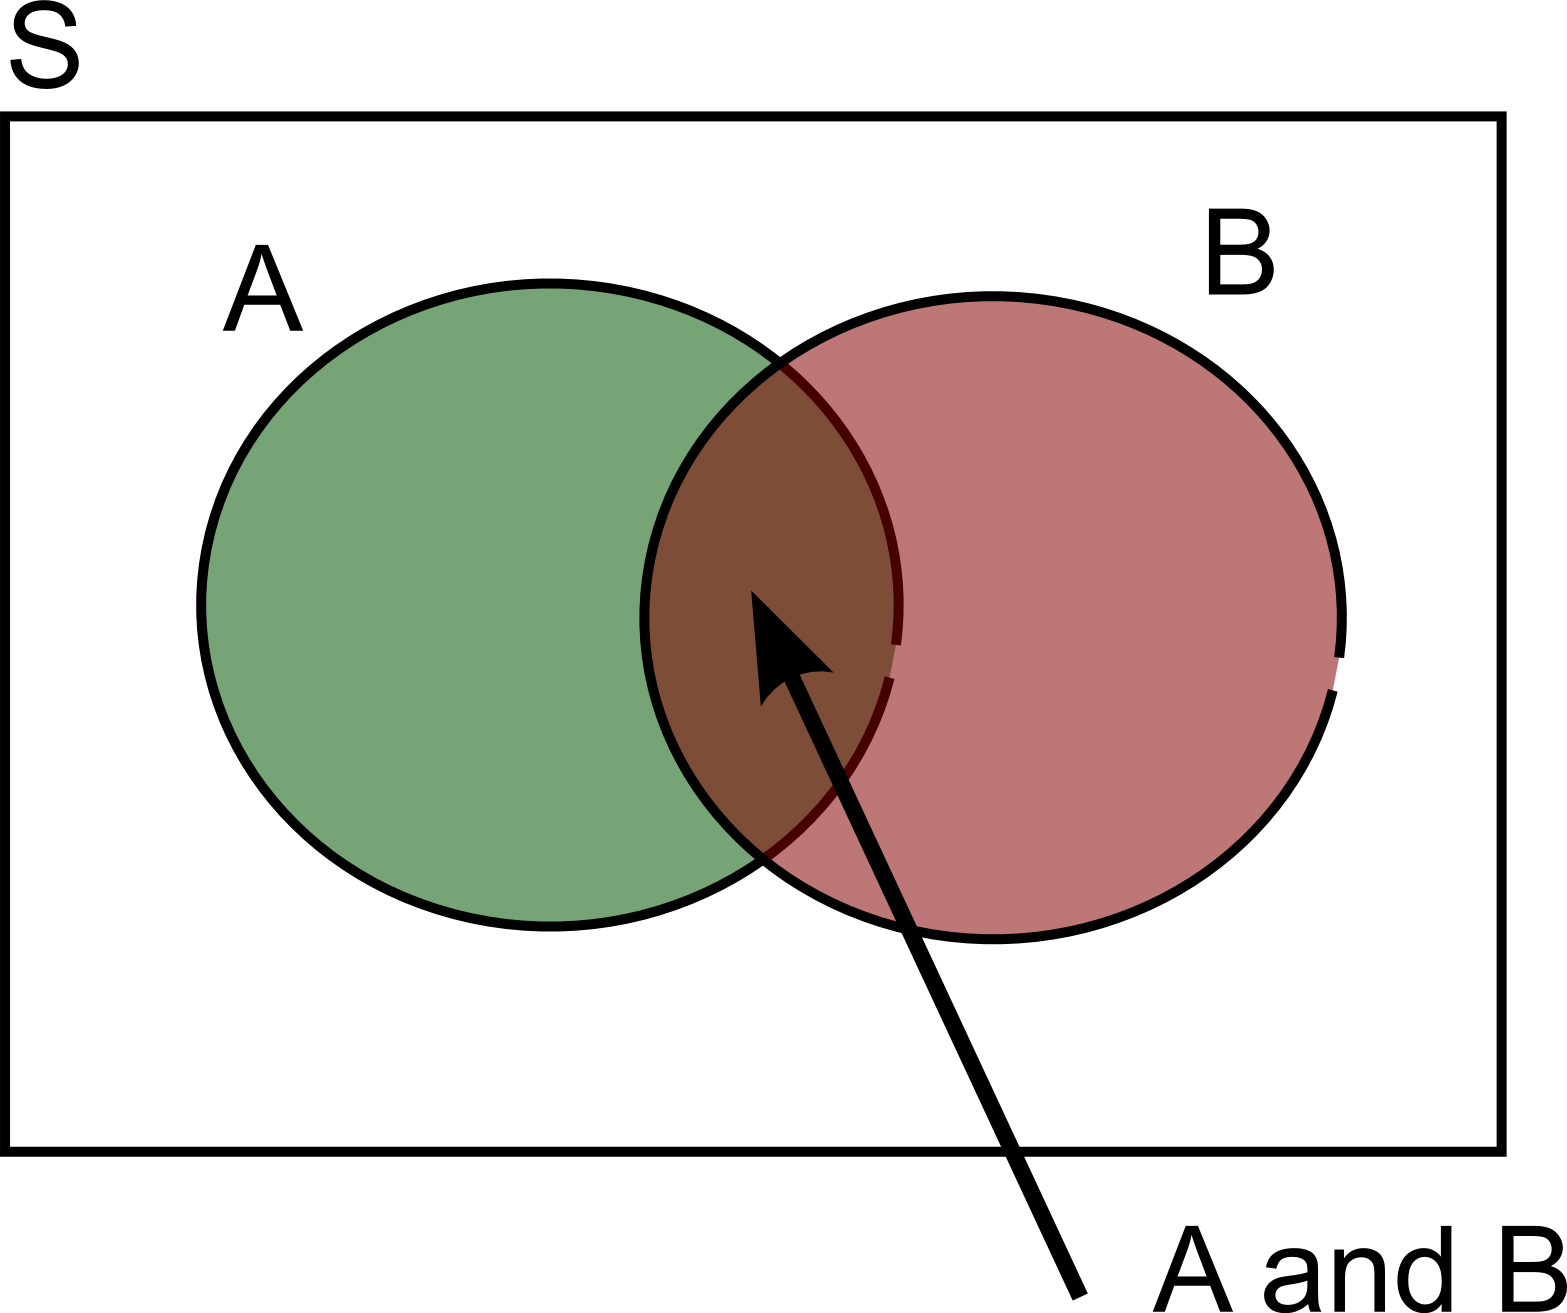
\includegraphics[width=5cm]{img/vennDiagramAnnotated}}
  \only<3->%
  {

    \begin{eqnarray*}
      p(\mathrm{A~or~B}) & = & p(A) + p(B) - p(\mathrm{A~and~B})
    \end{eqnarray*}
    Be careful about the discussion in the book about ``disjoint sets.''

  }
  
\end{frame}

\subsection{Compliment}

\begin{frame}{Compliment}

  The compliment of a set is everything not in the set.
  \only<1>{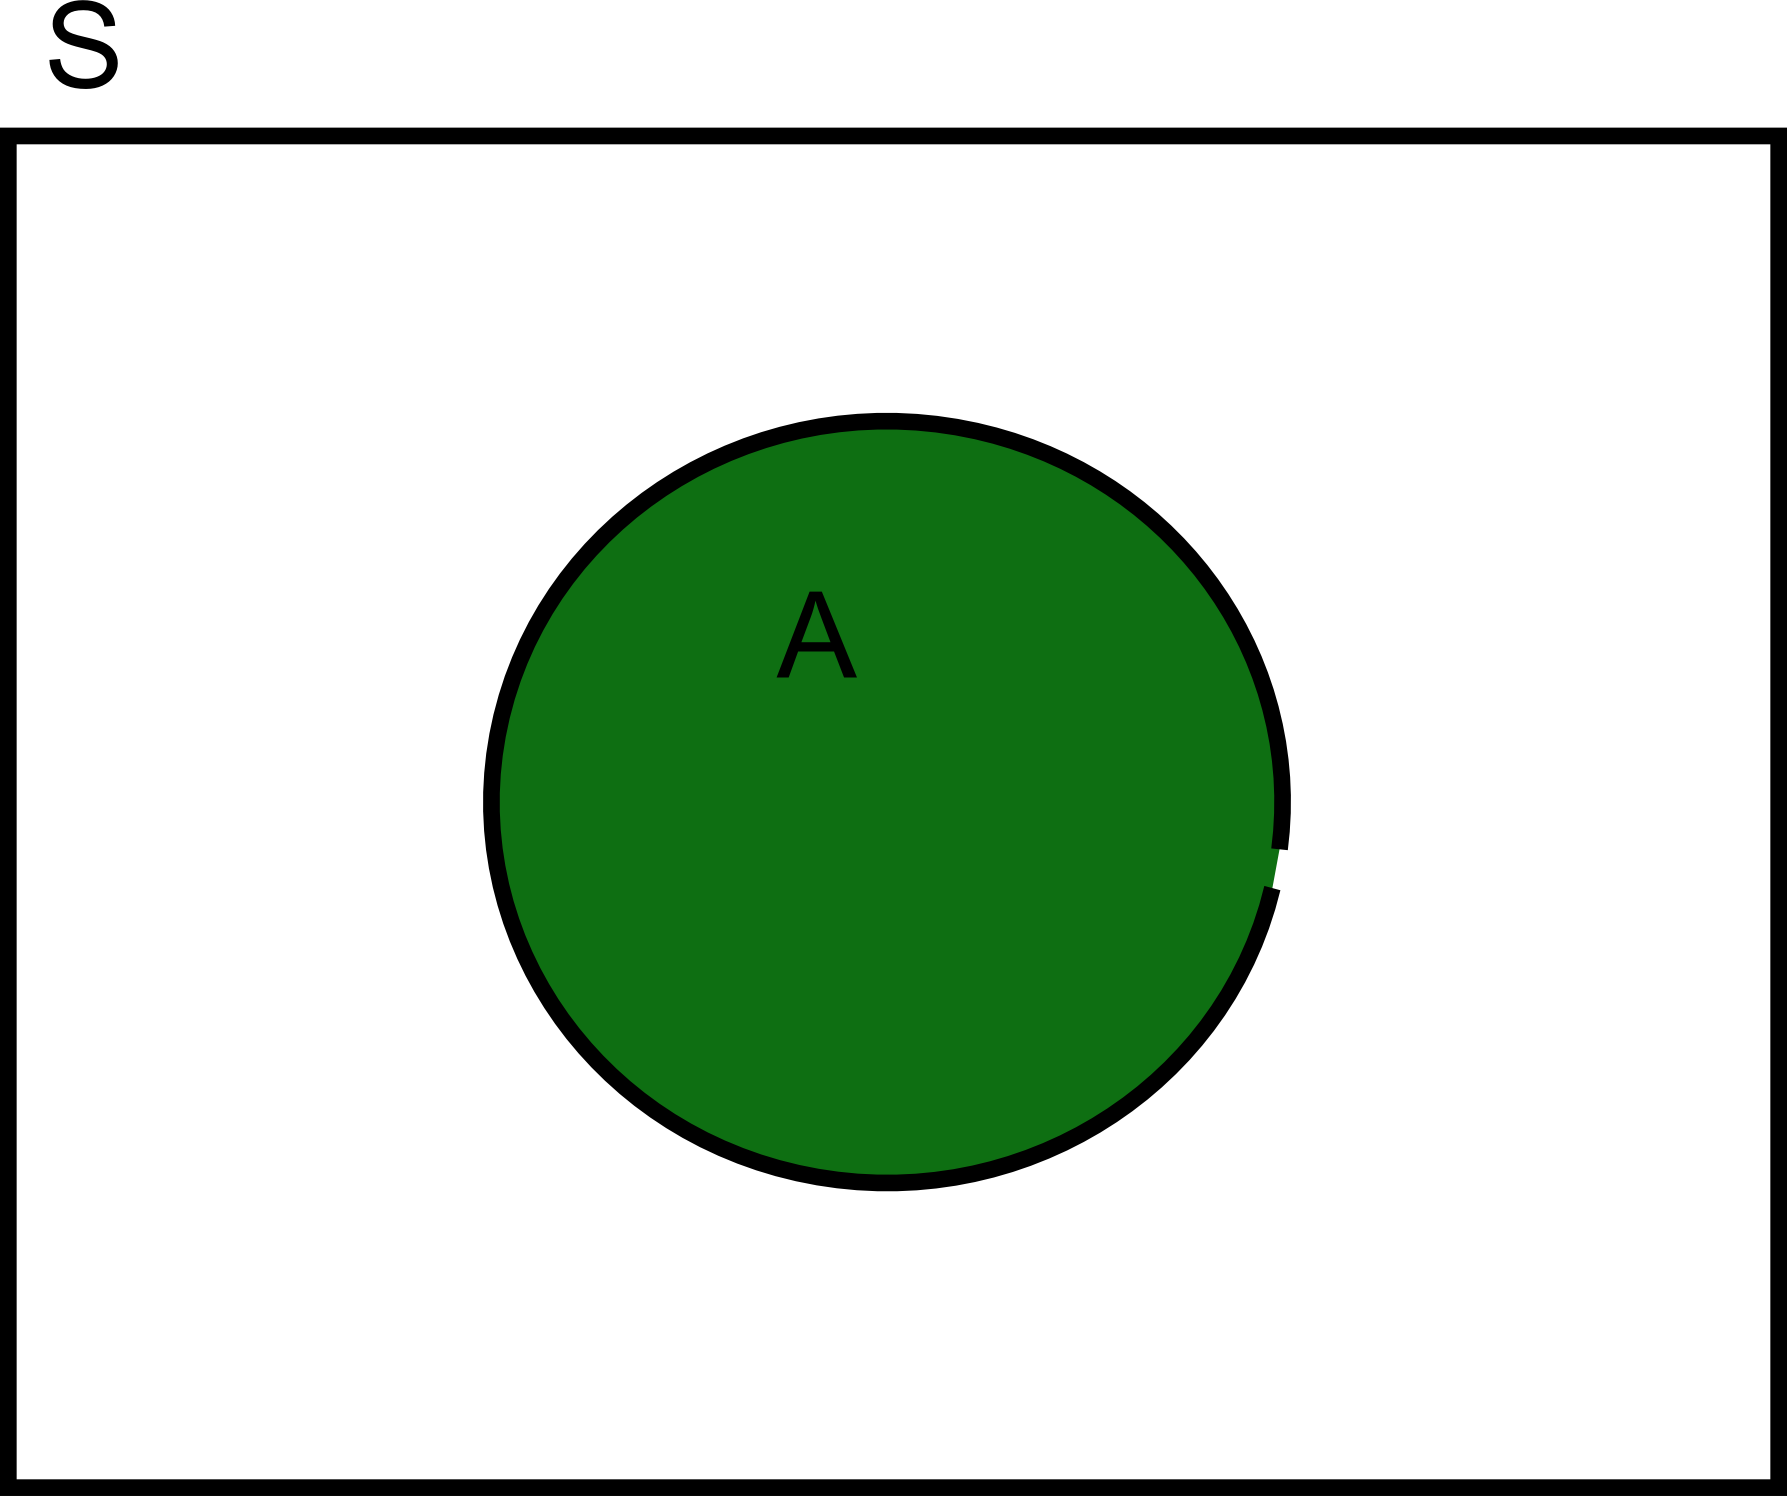
\includegraphics[width=5cm]{img/complimentVennOne}}
  \only<2>{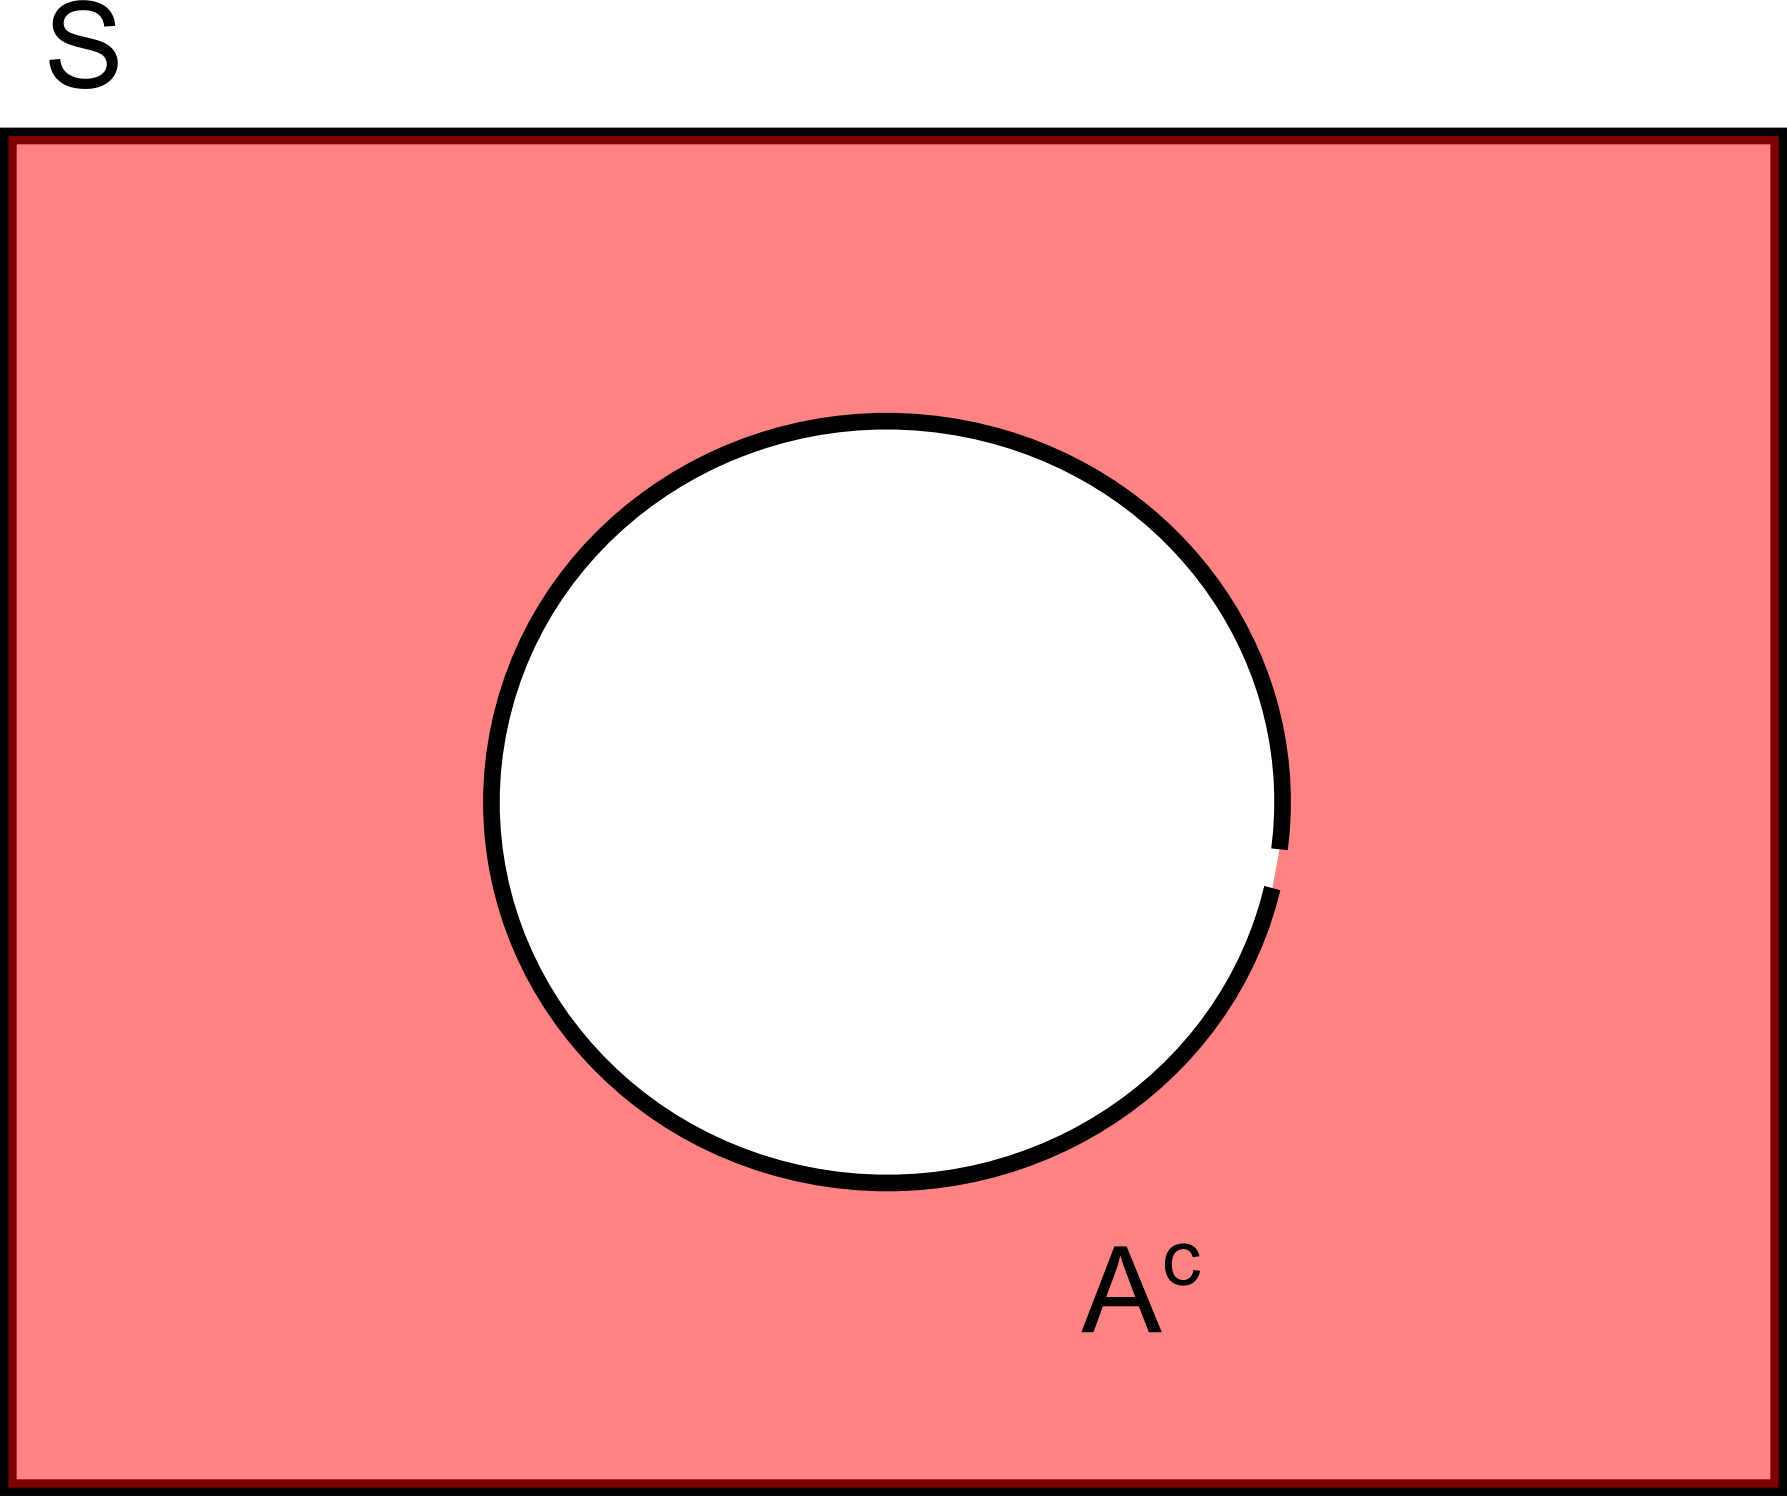
\includegraphics[width=5cm]{img/complimentVennTwo}}

  Notation:
  \begin{eqnarray*}
    A^c & = & \mathrm{Compliment~of~A}.
  \end{eqnarray*}

  
\end{frame}

\begin{frame}{Compliment}

  \begin{definition}
    Suppose $A$ is an event. Then all of the events not in A are denoted
    by $A^C$. 

    Other notations:
    \begin{eqnarray*}
      \bar{A},~A'.
    \end{eqnarray*}
  \end{definition}


\end{frame}




\begin{frame}{Probabilities of Compliments}
  
  \begin{eqnarray*}
    1 & = & p(A) + p(\bar{A}), \\
    p(A) & = & 1 - p(\bar{A}).
  \end{eqnarray*}

\end{frame}


\begin{frame}{Example}

  Number of drivers killed in fatal automobile crashes in 2005: \\
  \begin{tabular}{llll}
    Age & Male & Female & Total \\
    $<$16 & 227 & 77 & 304 \\
    16-20 & 5180 & 2113 & 7293 \\
    21-34 & 13611 & 4311 & 17922 \\
    35-54 & 15108 & 5027 & 20135 \\
    55-74 & 6801 & 2452 & 9253 \\
    $>$74   & 2022 & 980 & 3002 \\
    Total & 42949 & 14960 & 57909 
  \end{tabular} \\

  \vfill

  \textit{Traffic Safety Facts 2005, Federal Highway Administration,
    2005}

  \vfill

  I pick one person at random. What is the probability that the person
  is male and has an age between 21 and 34?

  
  
\end{frame}


\begin{frame}{Example}

  Number of drivers killed in fatal automobile crashes in 2005: \\
  \begin{tabular}{llll}
    Age & Male & Female & Total \\
    $<$16 & 227 & 77 & 304 \\
    16-20 & 5180 & 2113 & 7293 \\
    21-34 & \color{red}{13611} & 4311 & \color{green}{17922} \\
    35-54 & 15108 & 5027 & 20135 \\
    55-74 & 6801 & 2452 & 9253 \\
    $>$74   & 2022 & 980 & 3002 \\
    Total & \color{green}{42949} & 14960 & \color{red}{57909}
  \end{tabular} \\

  \vfill

  \textit{Traffic Safety Facts 2005, Fedoral Highway Administration,
    2005}

  \vfill

  I pick one person at random. What is the probability that the person
  is male {\color{blue}{\textbf{or}}} has an age between 21 and 34?

  
  
\end{frame}


\begin{frame}{Example}

  Number of drivers killed in fatal automobile crashes in 2005: \\
  \begin{tabular}{llll}
    Age & Male & Female & Total \\
    $<$16 & 227 & 77 & 304 \\
    16-20 & 5180 & 2113 & 7293 \\
    21-34 & 13611 & 4311 & 17922 \\
    35-54 & 15108 & 5027 & 20135 \\
    55-74 & 6801 & 2452 & 9253 \\
    $>$74   & 2022 & 980 & \color{green}{3002} \\
    Total & 42949 & 14960 & \color{green}{57909}
  \end{tabular} \\

  \vfill

  \textit{Traffic Safety Facts 2005, Federal Highway Administration,
    2005}

  \vfill

  I pick one person at random. What is the probability that the person's
  age is less than or equal to 74?

  
  
\end{frame}


\iftoggle{clicker}{%
  \begin{frame}{Clicker Quiz}

    Number of drivers killed in fatal automobile crashes in 2005: \\
    \begin{tabular}{llll}
      Age & Male & Female & Total \\
      $<$16 & 227 & 77 & 304 \\
      16-20 & 5180 & 2113 & 7293 \\
      21-34 & 13611 & 4311 & 17922 \\
      35-54 & 15108 & 5027 & 20135 \\
      55-74 & 6801 & 2452 & 9253 \\
      $>$74   & 2022 & 980 & 3002 \\
      Total & 42949 & 14960 & 57909 
    \end{tabular} \\

    \vfill

    \textit{Traffic Safety Facts 2005, Federal Highway Administration,
      2005}

    \vfill

    I pick one person at random. What is the probability that the person
    is female or age is between 16 and 20?

    \begin{tabular}{l@{\hspace{3em}}l@{\hspace{3em}}l@{\hspace{3em}}l}
      A: $\frac{2113}{57,909}$ & B:$\frac{14960}{57,909}$  \\ C:
      $\frac{2113}{57,909}+\frac{77}{57,909}$ &
      D: $\frac{14960}{57,909}+\frac{7293}{57,909}-\frac{2113}{57,909}$
    \end{tabular}
  
  
\end{frame}
}



\subsection{Conditional Probability}

\begin{frame}
  \frametitle{Example }

  1000 voters are polled in the 2008 election. We get the following
  information: \\
  \only<1>
  {
    \begin{tabular}{l|l|l|l}
      Education & Obama & McCain & Others  \\ \hline
      No H.S. Diploma & 19 & 20 & 1   \\
      H.S. Diploma only & 114 & 103 & 3 
    \end{tabular}
  }
  \only<2->
  {
    \begin{tabular}{l|l|l|l|l}
      Education & Obama & McCain & Others & Total \\ \hline
      No H.S. Diploma & 19 & 20 & 1 & 40 \\
      H.S. Diploma only & 114 & 103 & 3 & 220 \\ \hline
      Total & 133 & 123 & 4 & 260
    \end{tabular}
  }



\end{frame}


%\begin{frame}{Clicker Quiz}
%
%
%  A bowl has candy. Eight of the candies are chocolate, and of the
%  chocolates three have red wrappers while the rest have silver
%  wrappers. Twelve of the candies are hard candy, and of the hard
%  candies four have red wrappers while the rest have silver
%  wrappers. I pull out one candy at random, and it is a
%  chocolate. What is the probability that it has a red wrapper?
%
%  \begin{tabular}{l@{\hspace{3em}}l@{\hspace{3em}}l@{\hspace{3em}}l}
%    A: 4/12 & B: 3/8 & C: 5/8 & D: 8/12
%  \end{tabular}
%
%  
%\end{frame}




% LocalWords:  Clarkson pausesection hideallsubsections Obama
